\documentclass[12pt,a4paper]{article}
\usepackage[utf8]{inputenc}
\usepackage[spanish,es-tabla]{babel}
\usepackage{geometry}
\usepackage{graphicx}
\usepackage{multirow}
\usepackage{tabularx}
\usepackage{mathptmx}
\usepackage{fancyhdr}
\usepackage{array}
\usepackage[table]{xcolor}
\usepackage{titlesec}
\usepackage{setspace}
\usepackage{microtype}
\usepackage{lastpage}
\usepackage{booktabs}
\usepackage{enumitem}
\usepackage{amsmath}
\usepackage{amsfonts}
\usepackage{amssymb}

\usepackage{float}
\usepackage{placeins}
\usepackage{tikz}
\usepackage{pgfplots}
\pgfplotsset{compat=1.17}
\usetikzlibrary{arrows.meta,positioning,shapes.geometric,calc}

\graphicspath{{images/}{../images/}{./}}

\geometry{
    top=4.7cm,
    bottom=2.5cm,
    left=2.5cm,
    right=2.5cm,
    headheight=3.9cm,
    headsep=0.4cm
}

\setstretch{1.15}
\setlength{\parindent}{0pt}
\setlength{\parskip}{0.45em}
\setlength{\tabcolsep}{4pt}

\titleformat{\section}
  {\normalfont\fontsize{12}{14.5}\bfseries}{\thesection.}{0.6em}{\uppercase}
\titlespacing*{\section}
  {0pt}{1.8ex plus 0.4ex minus 0.2ex}{0.6ex plus 0.2ex}

\titleformat{\subsection}
  {\normalfont\fontsize{11.5}{13.5}\bfseries}{\thesubsection.}{0.5em}{}
\titlespacing*{\subsection}
  {0pt}{1.4ex plus 0.3ex minus 0.1ex}{0.4ex plus 0.1ex}

\titleformat{\subsubsection}
  {\normalfont\fontsize{10.5}{12.5}\bfseries\itshape}{\thesubsubsection.}{0.4em}{}
\titlespacing*{\subsubsection}
  {0pt}{1.1ex plus 0.2ex minus 0.1ex}{0.3ex plus 0.1ex}

\newcolumntype{Y}{>{\centering\arraybackslash}X}
\newcolumntype{L}{>{\raggedright\arraybackslash}X}
\newcolumntype{C}{>{\centering\arraybackslash}X}

\definecolor{headerblue}{RGB}{26, 54, 93}
\definecolor{darkblue}{RGB}{43, 108, 176}
\definecolor{lightgraybg}{RGB}{248, 248, 248}
\definecolor{tableheader}{RGB}{232, 238, 246}
\definecolor{navyheader}{RGB}{0, 32, 96}
\definecolor{lineblue}{RGB}{0, 102, 204}
\definecolor{areablue}{RGB}{220, 236, 252}
\definecolor{lcsred}{RGB}{217, 56, 41}
\definecolor{lcigreen}{RGB}{46, 125, 50}
\definecolor{lciorange}{RGB}{230, 81, 0}
\definecolor{ishikawared}{RGB}{160, 0, 0}

\tikzset{
    catbox/.style={draw, fill=tableheader, font=\footnotesize\bfseries, minimum width=2.8cm, minimum height=0.65cm, align=center},
    efectobox/.style={draw=ishikawared!90!black, line width=1.2pt, fill=ishikawared, text=white, font=\small\bfseries, align=center, inner sep=6pt, text width=3.8cm},
    causetext/.style={font=\scriptsize, align=right, text=black!90}
}

\newcommand{\docCodigo}{TI-SIGE-ENT-F1-002}
\newcommand{\docVersion}{1.0}
\newcommand{\docProceso}{INGENIERÍA DE REQUERIMIENTOS / STAKEHOLDERS Y PROCESOS}
\newcommand{\docElaboracion}{18/08/2026}
\newcommand{\docRevision}{18/08/2026}
\newcommand{\docTitulo}{IDENTIFICACIÓN DE ACTORES Y PROCESOS}
\newcommand{\docOrganizacion}{FACULTAD DE INGENIERÍA EN SISTEMAS, ELECTRÓNICA E INDUSTRIAL}
\newcommand{\docSubOrganizacion}{CARRERA DE INGENIERÍA DE SOFTWARE}

\newcommand{\encabezadofrecuente}{%
    \renewcommand{\arraystretch}{1.15}%
    \noindent\makebox[\textwidth][c]{%
    \begin{tabularx}{\textwidth}{|>{\centering\arraybackslash}m{2.8cm}|Y|>{\centering\arraybackslash}m{4.8cm}|}
        \hline
        \multirow{4}{2.8cm}{\centering\raisebox{-1.15cm}{
\includegraphics[width=2.5cm,height=2.0cm,keepaspectratio]{images/logo.png}}}
        & \textbf{\fontsize{9}{11}\selectfont \docOrganizacion} 
        & \textbf{\fontsize{8}{10}\selectfont CÓDIGO:} \fontsize{8}{10}\selectfont \docCodigo \\
        \cline{3-3}
        & \textbf{\fontsize{8.5}{10.5}\selectfont \docSubOrganizacion} 
        & \textbf{\fontsize{8}{10}\selectfont VERSIÓN:} \fontsize{8}{10}\selectfont \docVersion \\
        \cline{2-3}
        & \textbf{\fontsize{8}{10}\selectfont PROCESO:} \fontsize{8}{10}\selectfont \docProceso 
        & \textbf{\fontsize{8}{10}\selectfont ELABORACIÓN:} \fontsize{8}{10}\selectfont \docElaboracion \\
        \cline{2-3}
        & \textbf{\fontsize{8.5}{10.5}\selectfont \docTitulo} 
        & \textbf{\fontsize{8}{10}\selectfont ÚLTIMA REVISIÓN:} \fontsize{8}{10}\selectfont \docRevision \\
        \hline
    \end{tabularx}%
    }%
}

\pagestyle{fancy}
\fancyhf{}
\fancyhead[C]{\encabezadofrecuente}
\fancyfoot[C]{\fontsize{10}{12}\selectfont Página \thepage\ de \pageref{LastPage}}
\renewcommand{\headrulewidth}{0pt}

\begin{document}

\noindent{\fontsize{10.5}{12.5}\selectfont \textbf{Integrantes:} Heidi Villavicencio \quad$\vert$\quad Steeven Toala \quad$\vert$\quad Nixon Hurtado \quad$\vert$\quad Andrea Vásquez}

\vspace{0.25cm}

\section{Título}
\textbf{Denominación Oficial del Entregable:} Identificación de Actores y Procesos (Matriz de Stakeholders) -- Código EDT: 1.2

\section{Introducción}
El éxito en la implantación del sistema SIGE dentro de la FISEI requiere un análisis riguroso de los actores organizacionales que intervienen en el ciclo de vida de los planes de trabajo e informes institucionales. El Sistema de Gestión de Calidad establece una cadena jerárquica con responsabilidades claramente delimitadas, desde la docencia de aula hasta las autoridades de facultad. El presente informe formaliza el mapa de interesados (\textit{Stakeholders}) y clasifica sus niveles de poder e interés para fundamentar la matriz de control de acceso y perfiles del sistema.

\section{Objetivo}
\subsection{Objetivo General}
Identificar, mapear y caracterizar formalmente a los actores organizacionales y los macroprocesos institucionales que interactúan con el Sistema de Gestión de Calidad en la FISEI, estructurando la Matriz de Stakeholders del proyecto SIGE.
\subsection{Objetivos Específicos}
\begin{itemize}[leftmargin=1.5em, itemsep=2pt]
    \item Identificar las funciones institucionales de los roles: Docente Elaborador, Coordinador de Área, Coordinador de Carrera, Subdecano y Administrador SGC.
    \item Analizar la matriz de Poder versus Interés según la metodología estándar del PMBOK.
    \item Modelar la asignación de responsabilidades mediante la matriz RACI de la cadena documental.
\end{itemize}

\section{Alcance}
\subsection{Límites del Entregable (In-Scope)}
\begin{itemize}[leftmargin=1.5em, itemsep=2pt]
    \item Mapeo de interesados en las cuatro carreras de la FISEI (Software, TI, Telecomunicaciones, Computación).
    \item Asignación de responsabilidades para el flujo documental de planificación semestral y rendición de cuentas.
\end{itemize}
\subsection{Exclusiones (Out-of-Scope)}
\begin{itemize}[leftmargin=1.5em, itemsep=2pt]
    \item Personal administrativo externo al Decanato y Subdecanato de la FISEI.
\end{itemize}

\section{Definiciones}
\begin{itemize}[leftmargin=1.5em, itemsep=2pt]
    \item \textbf{Stakeholder (Interesado):} Individuo o grupo que puede afectar, verse afectado o percibirse como afectado por una decisión, actividad o resultado del proyecto.
    \item \textbf{Matriz RACI:} Modelo de asignación de responsabilidades que clasifica la participación de los actores en: Responsable (\textit{R}), Aprobador (\textit{A}), Consultado (\textit{C}) e Informado (\textit{I}).
    \item \textbf{Comisión Académica:} Órgano colegiado de carrera encargado de auditar la pertinencia de las actividades y medios de verificación docentes.
\end{itemize}

\section{Responsabilidades}
\begin{itemize}[leftmargin=1.5em, itemsep=2pt]
    \item \textbf{Nixon Hurtado (Responsable EDT 1.2):} Identificación de roles y caracterización de procesos.
    \item \textbf{Andrea Vásquez (Analista de Procesos):} Construcción de la matriz RACI y diagramas de interacción.
    \item \textbf{Ing. Paulo Torres (Docente Evaluador):} Aprobación del mapa institucional de actores.
\end{itemize}

\section{Normativa Legal y Técnica}
\subsection{Marco Legal Ecuatoriano}
\begin{itemize}[leftmargin=1.5em, itemsep=2pt]
    \item \textbf{Estatuto Orgánico de la Universidad Técnica de Ambato:} Atribuciones de subdecanos, directores y coordinadores de carrera.
    \item \textbf{Ley Orgánica de Educación Superior (LOES), Art. 122.}
\end{itemize}
\subsection{Normas Técnicas Internacionales}
\begin{itemize}[leftmargin=1.5em, itemsep=2pt]
    \item \textbf{PMBOK Guide (7th Edition):} Gestión de interesados y análisis de expectativas.
    \item \textbf{ISO 9001:2015, Cláusula 5.3 (Roles, responsabilidades y autoridades en la organización).}
\end{itemize}

\section{Método, Políticas y Contenidos}
\subsection{Enfoque Metodológico}
Se aplicó el modelo de categorización de interesados del PMI, evaluando a los 5 roles clave según su nivel de autoridad formal e interés operativo en el sistema. Asimismo, se documentaron los macroprocesos de Gestión Curricular y Aseguramiento de la Calidad.

\subsection{Políticas de Gestión de Interesados}
\begin{enumerate}[leftmargin=1.5em, itemsep=2pt]
    \item \textbf{Política de Segregación de Funciones:} El docente elaborador no puede auto-aprobarse ni revisar su propio plan de trabajo.
    \item \textbf{Política de Jerarquía de Firma:} La firma del Subdecano solo puede registrarse tras el visado formal del Coordinador de Carrera.
    \item \textbf{Política de Notificación Inmediata:} Cualquier observación emitida por el comité debe notificarse automáticamente al docente.
\end{enumerate}

\section{Descripción de actividades}
La correcta asignación de responsabilidades y la eliminación de etapas de aprobación redundantes constituyeron el eje de las actividades de ingeniería de procesos ejecutadas en la facultad. El equipo técnico llevó a cabo las siguientes actividades de modelado organizacional:

\begin{itemize}[leftmargin=1.5em, itemsep=4pt]
    \item \textbf{Análisis de Competencias Orgánicas y Marco Estatutario UTA/LOES:} Se revisó el Estatuto de la Universidad Técnica de Ambato y el Reglamento de Régimen Académico (RRA - CES) para deslindar con precisión las atribuciones jurídicas de cada rol. Se determinó que el Coordinador de Comisión posee competencia de revisión técnica y disciplinar, mientras que el Subdecano de Facultad ostenta la autoridad legal exclusiva para la aprobación institucional final.
    \item \textbf{Taller de Mapeo de Interacciones y Flujos de Decisión Inter-departamentales:} Se desarrolló una sesión de trabajo colaborativo junto a los coordinadores de carrera y comisiones académicas de la FISEI, modelando formalmente los cinco roles esenciales del sistema: Docente Elaborador, Coordinador de Comisión, Director de Carrera, Subdecano de Facultad y Administrador del SGC, eliminando dos revisiones informales que generaban duplicidad sin valor agregado.
    \item \textbf{Estructuración de la Matriz RACI Institucional del Ciclo Documental:} Para cada una de las 8 fases del flujo documental (Configuración Inicial, Carga Horaria, Redacción Descriptiva, Matriz Dinámica, Custodia de Evidencias, Revisión Técnica de Comisión, Aprobación de Subdecanato y Custodia Histórica), se asignó con rigor quién es Responsable de ejecutar (R), Quién Aprueba legalmente (A), A quién se Consulta técnicamente (C) y Quién debe ser Informado (I).
    \item \textbf{Segmentación y Evaluación de Involucrados según el Marco PMBOK:} Se clasificaron los actores institucionales mediante una matriz de Poder versus Interés, definiendo estrategias diferenciadas de comunicación, vistas de tablero con permisos RBAC y canales de notificación asíncrona adaptados a su nivel de dedicación horaria.
\end{itemize}

\subsection{Matriz RACI de la Cadena Documental Institucional}
\begin{table}[H]
\centering
\small
\renewcommand{\arraystretch}{1.2}
\begin{tabularx}{\textwidth}{|>{\hsize=1.5\hsize\raggedright\arraybackslash\bfseries\footnotesize}X|>{\hsize=0.9\hsize\centering\arraybackslash\footnotesize}X|>{\hsize=0.9\hsize\centering\arraybackslash\footnotesize}X|>{\hsize=0.9\hsize\centering\arraybackslash\footnotesize}X|>{\hsize=0.9\hsize\centering\arraybackslash\footnotesize}X|>{\hsize=0.9\hsize\centering\arraybackslash\footnotesize}X|}
\hline
\rowcolor{tableheader}
\textbf{Actividad del Proceso SGC} & \textbf{Docente} & \textbf{Coord. Área} & \textbf{Coord. Carrera} & \textbf{Subdecano} & \textbf{Admin SGC} \\
\hline
Creación y Llenado del Plan P7-T1 & \textbf{R / A} & C & I & I & I \\
\hline
Revisión Técnica y Observaciones & I & \textbf{R} & \textbf{R / A} & I & I \\
\hline
Subsanación de Observaciones & \textbf{R / A} & C & C & I & I \\
\hline
Aprobación y Firma de Comisión & I & C & \textbf{R / A} & I & I \\
\hline
Legalización en Consejo Directivo & I & I & I & \textbf{R / A} & I \\
\hline
Apertura de Prórrogas y Catálogos & I & I & C & C & \textbf{R / A} \\
\hline
\end{tabularx}
\caption{Matriz RACI oficial de la cadena de responsabilidades SGC.}
\label{tab:matriz_raci}
\end{table}

\section{Firmas de Responsabilidad}

\noindent
\renewcommand{\arraystretch}{1.2}%
\begin{tabularx}{\textwidth}{|>{\hsize=0.7\hsize\raggedright\arraybackslash}X|>{\hsize=1.4\hsize\raggedright\arraybackslash}X|>{\hsize=1.2\hsize\centering\arraybackslash}X|>{\hsize=0.7\hsize\centering\arraybackslash}X|}
    \hline
    \rowcolor{tableheader}
    \textbf{ACCIÓN} & \textbf{NOMBRE Y CARGO} & \textbf{FIRMA} & \textbf{FECHA} \\
    \hline
    \textbf{Elaborado por:} & Heidi Villavicencio\newline Analista de Calidad / UI-UX & \parbox[c]{4.4cm}{\centering\vspace{4pt}
\includegraphics[height=1.5cm,width=4.0cm,keepaspectratio]{images/firma_heidi.png}\vspace{4pt}} & 18/08/2026 \\
    \hline
    \textbf{Revisado por:} & Steeven Toala\newline Líder de Proyecto / Arquitecto & \parbox[c]{4.4cm}{\centering\vspace{4pt}
\includegraphics[height=1.5cm,width=4.0cm,keepaspectratio]{images/firma_steveen.png}\vspace{4pt}} & 18/08/2026 \\
    \hline
    \textbf{Aprobado por:} & Ing. Paulo Torres, Mg.\newline Docente Evaluador -- Gestión Proyectos & \parbox[c]{4.4cm}{\centering\vspace{8pt}\textbf{\textcolor{gray!80}{\scriptsize [ PENDIENTE DE APROBACIÓN ]}}\vspace{8pt}} & \textbf{\textcolor{gray!90}{Pendiente}} \\
    \hline
\end{tabularx}%

\vspace{0.4cm}

\section{Control de Cambios}

\noindent
\renewcommand{\arraystretch}{1.2}
\begin{tabularx}{\textwidth}{|>{\hsize=0.45\hsize\centering\arraybackslash}X|>{\hsize=1.55\hsize\raggedright\arraybackslash}X|>{\hsize=1.2\hsize\raggedright\arraybackslash}X|>{\hsize=0.8\hsize\centering\arraybackslash}X|}
    \hline
    \rowcolor{tableheader}
    \textbf{Versión} & \textbf{Descripción del cambio} & \textbf{Responsable del cambio} & \textbf{Fecha de aprobación} \\
    \hline
    1.0 & Elaboración de la matriz de partes interesadas (Stakeholders), asignación de niveles RACI y perfiles de usuario. & Heidi Villavicencio / Nixon Hurtado & 18/08/2026 \\
    \hline
\end{tabularx}

\vspace{0.4cm}

\section{Anexos}

\subsection*{Anexo: Evidencias de Mapeo de Actores y Macroprocesos Institucionales}

\subsubsection*{1. Análisis de Competencias Orgánicas y Modelado de Roles del SGC}
La identificación de actores y macroprocesos no se basó en supuestos teóricos, sino en el organigrama funcional y el estatuto orgánico de la Universidad Técnica de Ambato, así como en las 14 comisiones oficiales activas en la FISEI documentadas en el catálogo institucional.

El proceso de caracterización se estructuró de la siguiente forma:
\begin{enumerate}[leftmargin=1.5em, itemsep=2pt]
    \item \textbf{Delimitación de Competencias y Atribuciones Estatutarias:} Se mapearon las funciones según la Ley Orgánica de Educación Superior (LOES) y el Reglamento de Régimen Académico (RRA). Se definieron formalmente cinco roles de interacción: Docente Elaborador (autor del plan e informe), Coordinador de Comisión (revisor de actividades específicas), Coordinador de Carrera (primer filtro académico colegiado), Subdecano (auditor de carga horaria y comisiones) y Administrador SGC (gestor de periodos y catálogos).
    \item \textbf{Construcción y Asignación de la Matriz RACI Institucional:} Se clasificaron las responsabilidades en Responsable (\textit{R}), Aprobador (\textit{A}), Consultado (\textit{C}) e Informado (\textit{I}) para cada una de las 6 fases del ciclo de calidad, evitando la duplicidad de funciones identificada en el proceso As-Is.
    \item \textbf{Análisis de Involucrados Mediante Matriz de Poder versus Interés:} Se categorizó a cada grupo de interés para definir la estrategia de gestión del cambio tecnológico y diseño de interfaces.
\end{enumerate}

\subsubsection*{2. Evidencia Visual del Mapa de Macroprocesos y Explicación Técnica}
\begin{figure}[H]
    \centering
    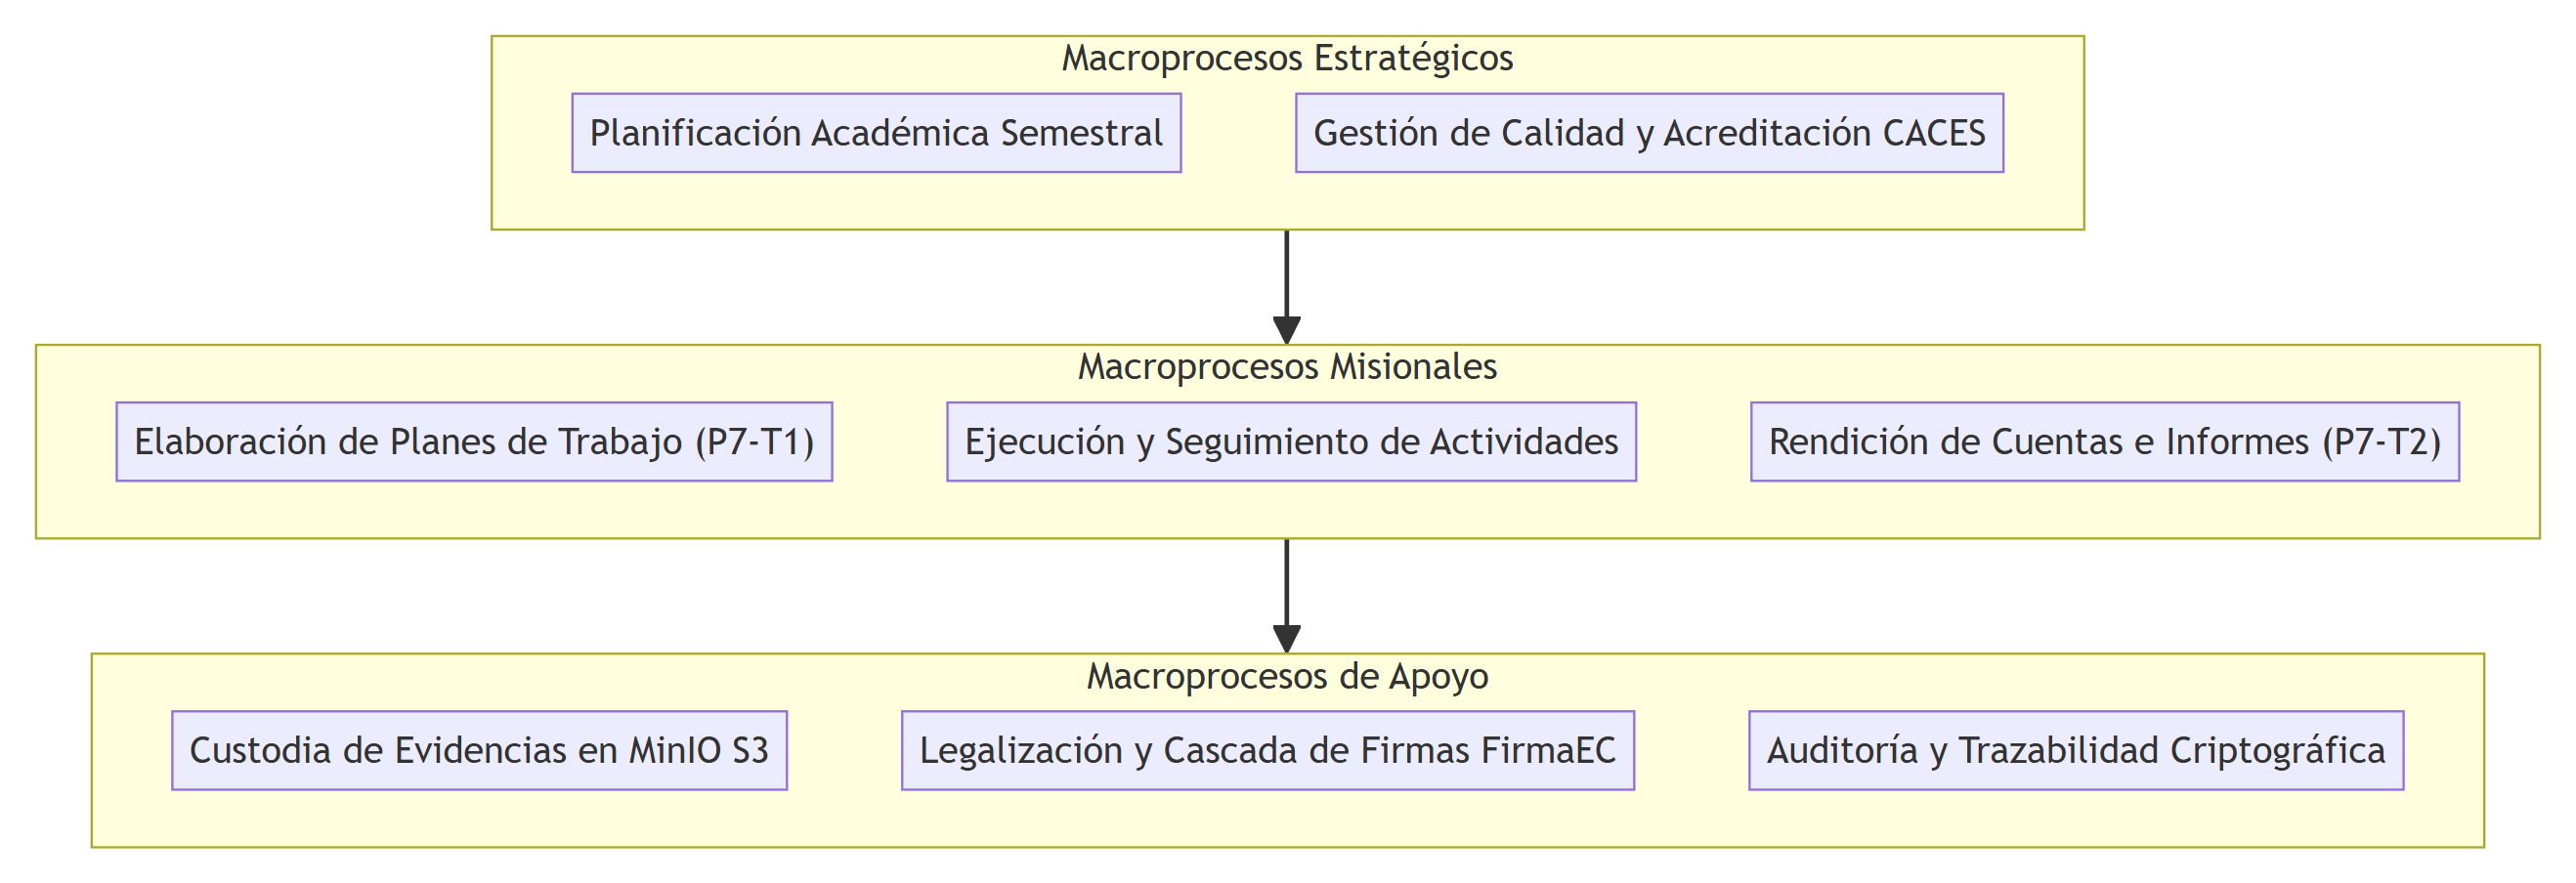
\includegraphics[width=0.92\textwidth,keepaspectratio]{images/s1_02_macroprocesos.png}
    \caption{Mapa de Macroprocesos Institucionales del SGC y Cadena de Valor Docente en FISEI.}
    \label{fig:macroprocesos}
\end{figure}
\FloatBarrier

\noindent
\noindent
\textbf{Desglose Técnico y Análisis Estructural de Macroprocesos y Actores:}
\begin{itemize}[leftmargin=1.5em, itemsep=3pt]
    \item \textbf{Jerarquía de Procesos Estratégicos, Misionales y de Soporte:} La arquitectura del mapa articula tres niveles operativos: en el nivel estratégico se sitúan las Directrices del Honorable Consejo Directivo y Subdecanato; en el nivel misional central se ubica la Elaboración y Seguimiento del Plan de Trabajo Docente (\texttt{P7-\allowbreak T1}) y Cumplimiento (\texttt{P7-\allowbreak T4}); y en el nivel de soporte se integran la Secretaría Académica y la Custodia Documental.
    \item \textbf{Interacción de Roles Institucionales y Cadena de Valor:} El diagrama desglosa los 5 perfiles formales del sistema: Docente Elaborador (origen de datos), Coordinador de Comisión (revisión disciplinar), Director de Carrera (consolidación de programas), Subdecano (legalización y fiscalización de 40h) y Administrador SGC (parametrización de periodos y carreras).
    \item \textbf{Alineación con la Matriz RACI Institucional:} El mapa delimita con precisión que la responsabilidad de ejecución (\textit{R}) recae en el docente, mientras que la autoridad de aprobación final (\textit{A}) corresponde legalmente al Subdecano, eliminando pasos redundantes de visto bueno informal que ralentizaban el proceso.
    \item \textbf{Implementación en el Sistema SIGE:} Este mapa define la estructura del control de acceso basado en roles (RBAC) en el backend de Express v5 y las vistas del enrutador en React, garantizando que cada usuario acceda únicamente a las opciones correspondientes a su perfil.
\end{itemize}

\subsubsection*{3. Matriz RACI Oficial de Responsabilidades en el Ciclo Documental SGC}
\begin{table}[H]
\centering
\small
\renewcommand{\arraystretch}{1.2}
\begin{tabularx}{\textwidth}{|>{\hsize=1.2\hsize\raggedright\arraybackslash\bfseries\footnotesize}X|>{\hsize=0.7\hsize\centering\arraybackslash\footnotesize}X|>{\hsize=0.7\hsize\centering\arraybackslash\footnotesize}X|>{\hsize=0.7\hsize\centering\arraybackslash\footnotesize}X|>{\hsize=0.7\hsize\centering\arraybackslash\footnotesize}X|}
\hline
\rowcolor{tableheader}
\textbf{Fase del Proceso SGC} & \textbf{Docente} & \textbf{Comisión} & \textbf{Coordinador} & \textbf{Subdecano} \\
\hline
1. Elaboración y Registro del Plan (P7-T1) & \textbf{R / A} & C & I & I \\
\hline
2. Verificación de Carga Horaria (40h) & R & C & \textbf{R} & \textbf{A} \\
\hline
3. Seguimiento Semestral de Actividades & \textbf{R} & C & I & I \\
\hline
4. Carga y Custodia de Evidencias en S3 & \textbf{R} & C & C & I \\
\hline
5. Revisión Colegiada de Cumplimiento & I & \textbf{R} & \textbf{R / A} & C \\
\hline
6. Aprobación y Legalización de Firmas & R & C & R & \textbf{R / A} \\
\hline
\end{tabularx}
\caption{Matriz RACI formal de responsabilidades para el sistema SIGE.}
\end{table}


\end{document}
